%%%%%%%%%%%%%%%%%%%%%%%%%%%%%%%%%%%%%%%%%%%%%%%%%%%%%%%%%%%%%%%%%%%%%%%%%%%%%%%
\section{\orangebold{Part 2.} Improving the Robustness of Convolutional Neural Networks}
%%%%%%%%%%%%%%%%%%%%%%%%%%%%%%%%%%%%%%%%%%%%%%%%%%%%%%%%%%%%%%%%%%%%%%%%%%%%%%%



%%%%%%%%%%%%%%%%%%%%%%%%%%%%%%%%%%%%%%%%%%%%%%%%%%%%%%%%%%%%%%%%%%%%%%%%%%%%%%%
\begin{frame}{Crafting Adversarial Attacks}
%%%%%%%%%%%%%%%%%%%%%%%%%%%%%%%%%%%%%%%%%%%%%%%%%%%%%%%%%%%%%%%%%%%%%%%%%%%%%%%

  An \textbf{Adversarial Attack} aims at finding a \orangebold{perturbation} $\tau$ such that:
  \begin{itemize}
      \item[$\bullet$] the network misclassifies
      \item[$\bullet$] $\norm{\tau}_p \leq \epsilon$ where $\epsilon$ is small
  \end{itemize}

  \begin{minipage}{\textwidth}
    \centering
    \begin{minipage}{0.45\textwidth}
      Finding the perturbation $\tau$ can be formalized by:
      \begin{equation}
	\tau^{\mathrm{adv}}(\xvec, y; h) \triangleq \argmax_{\norm{\tau}_p \leq \epsilon} \ell(h(\xvec + \tau), y)
      \end{equation}
    \end{minipage}
    \hfill
    \begin{minipage}{0.49\textwidth}
      \centering
      \begin{overpic}[scale=0.3]{images/adv_example/adv_example.pdf}
        \put (42, 53) {\scalebox{1.8}{$\tau$}}
        \put (68, 69) {\scalebox{1.}{$h(\xvec) = y$}}
	\put (68, 84) {\scalebox{1.}{$h(\xvec) \neq y$}}
      \end{overpic}
    \end{minipage}
  \end{minipage}

\end{frame}





%%%%%%%%%%%%%%%%%%%%%%%%%%%%%%%%%%%%%%%%%%%%%%%%%%%%%%%%%%%%%%%%%%%%%%%%%%%%%%%
\begin{frame}{Defending against Adversarial Attacks}
%%%%%%%%%%%%%%%%%%%%%%%%%%%%%%%%%%%%%%%%%%%%%%%%%%%%%%%%%%%%%%%%%%%%%%%%%%%%%%%

  One of the best empirical defense against adversarial attacks is to minimize the \orangebold{Empirical Adversarial Risk} ({\color{SkyBlue}{\cite{goodfellow2014explaining}}}): 
  \begin{equation}
    \hat{R}^{\mathrm{adv}}_m(h) \triangleq \frac{1}{m} \sum_{m=1}^{m} \ell \left( h(\xvec_i + \tau^{\mathrm{adv}}(\xvec_i, y_i; h)), y_i \right)
  \end{equation}

  \visible<2->{
    We can bound the adversarial risk by the empirical adversarial risk and a complexity penalty:
    \begin{equation}
      R^{\mathrm{adv}}(h) \quad \leq \quad \hat{R}^{\mathrm{adv}}_m(h) \quad +  \quad \underbrace{P^{\mathrm{adv}}(h)}_{\text{Complexity}\atop\text{Penalty}}
    \end{equation}
  }

  \vspace{-0.4cm}
  \visible<2->{
    The \orangebold{Adversarial Complexity Penalty} depends on the Lipschitz constant of the network ({\color{SkyBlue}{\citet{farnia2018generalizable}}}).
  }

  \vspace{0.2cm}
  \visible<3->{
    \begin{mdframed}[linecolor=OrangePSL,linewidth=1pt]
      \centering
      Reducing the Lipschitz constant of the Neural Network improves the robustness against adversarial attacks.
    \end{mdframed}
  }

  
\end{frame}



%%%%%%%%%%%%%%%%%%%%%%%%%%%%%%%%%%%%%%%%%%%%%%%%%%%%%%%%%%%%%%%%%%%%%%%%%%%%%%%
\begin{frame}{Bounding the Lipschitz Constant of Neural Networks}
%%%%%%%%%%%%%%%%%%%%%%%%%%%%%%%%%%%%%%%%%%%%%%%%%%%%%%%%%%%%%%%%%%%%%%%%%%%%%%%

  Combining Adversarial Training and Lipschitz regularization: 

  \begin{equation}
    \argmin_{h \in \Hcal} \ \frac{1}{m} \sum_{i = 1}^{m} \underbrace{\vphantom{\frac{1}{1}} \ell \left( h (\xvec_i + \tau^{\mathrm{adv}}(\xvec_i, y_i; h)), y_i \right)}_{\text{Adversarial Training}} \quad + \quad \underbrace{ \vphantom{\frac{1}{1}} \lambda \lip(h)}_{\text{Lipschitz Regularization}}
  \end{equation}

  \begin{minipage}{\textwidth}
    \centering
    \begin{tikzpicture}[overlay]
      \visible<2->{
	\node (myrec) at (3.6,1.2) [rectangle,draw,color=OrangePSL,thick,minimum width=2.5cm,minimum height=1.3cm] {};
	\node[above,yshift=0] at (myrec.north) {
          \begin{minipage}{0.35\textwidth}
            \centering
            {\small{\orangebold{NP-hard problem}}} \\[-0.2cm]
            {\tiny{{\color{SkyBlue}{\cite{scaman2018lipschitz}}}}}
          \end{minipage}
         }
      ;}
    \end{tikzpicture}
  \end{minipage}

  \vspace{-0.5cm}
  \visible<3->{
    \begin{minipage}{\textwidth}
      \centering
      \begin{tikzpicture}
	\node (main) at (0, 0) {$\text{Bounding } \lip(h)$};
	\visible<4->{
	\node (left) at ([shift={(-1cm,-1.5cm)}]main.west) {
	  \begin{minipage}{0.45\textwidth}
	    \centering
	    {\footnotesize
	    \textbf{Tight bound on the Lipschitz}
	    \begin{itemize}[itemsep=0pt,parsep=0pt,topsep=0pt]
	     \item[$\bullet$] Autograd \\ \vspace{-0.1cm} {\tiny{{\color{SkyBlue}{\cite{scaman2018lipschitz}}}}}
	     \item[$\bullet$] Semi-definite Programming \\ \vspace{-0.1cm} {\tiny{{\color{SkyBlue}{\cite{fazlyab2019efficient}}}}}
	    \end{itemize}
	     }
	  \end{minipage}
	};}
	\visible<5->{
	\node (right) at ([shift={(+1cm,-1.5cm)}]main.east) {
	  \begin{minipage}{0.45\textwidth}
	    \begin{equation}
	      \lip(h) \leq \prod_{i=1}^p \sigma_1\left(\Wmat^{(i)}\right)
	    \end{equation}
	  \end{minipage}
	};}
	  \visible<4->{
	  \path[OrangePSL,thick,->] (main.south west) edge [bend right] (left.north);
	}
	\visible<5->{
	  \path[OrangePSL,thick,->] (main.south east) edge [bend left] (right.north);
	}
      \end{tikzpicture}
    \end{minipage}
  }

  \vspace{0.2cm}
  \visible<6->{
    \begin{mdframed}[linecolor=OrangePSL,linewidth=1pt]
      \centering
      \textbf{Goal}: Exploit the properties of convolutions to find a fast and accurate approximation of their largest singular values.
    \end{mdframed}
  }
 
\end{frame}







%%%%%%%%%%%%%%%%%%%%%%%%%%%%%%%%%%%%%%%%%%%%%%%%%%%%%%%%%%%%%%%%%%%%%%%%%%%%%%%
\begin{frame}{Fourier analysis for Toeplitz Matrices}
%%%%%%%%%%%%%%%%%%%%%%%%%%%%%%%%%%%%%%%%%%%%%%%%%%%%%%%%%%%%%%%%%%%%%%%%%%%%%%%


  We can easily bound the largest singular value of Toeplitz matrices

  \begin{theorem}[{\color{SkyBlue}{\cite{gray2006toeplitz}}}\xspace]
    Let $\Tmat$ be a Toeplitz matrix and $f$ be the inverse Fourier Transform of the Toeplitz sequence, then:
    \begin{equation}
      \sigma_1 \left( \Tmat \right) \leq \sup_{\omega \in [0, 2\pi]} |f(\omega)|
    \end{equation}
  \end{theorem}

  In this result, $f:[0, 2\pi] \rightarrow \Cbb$ is a complex-valued function of the following form:

  \begin{minipage}{\textwidth}
    \centering
    \vspace{-0.3cm}
    \begin{minipage}{0.45\textwidth}
      \begin{equation}
	  \Tmat = \scalebox{0.8}{
	  \begin{tikzpicture}[
	    baseline,
	    every left delimiter/.style={xshift=+0.78em},
	    every right delimiter/.style={xshift=-0.4em},
	    mymat/.style={
	      matrix of math nodes,
	      ampersand replacement=\&,
	      left delimiter=(,
	      right delimiter=),
	      nodes={
		text depth=0.5ex,
		text height=2ex,
		text width=2em,
		align=center}
	    }
	    ]
	    \matrix[mymat] (mytoeplitz) {
	       \asf_0  \& \asf_1 \& \cdots \& \asf_{n-1} \\
	       \asf_{-1} \& \color{black!30}{\asf_0} \& \color{black!30}{\ddots} \& \color{black!30}{\vdots} \\
	       \vdots  \& \color{black!30}{\ddots}  \& \color{black!30}{\asf_0}    \& \color{black!30}{\asf_1} \\
	       \asf_{-n+1} \& \color{black!30}{\cdots}  \& \color{black!30}{\asf_{-1}} \& \color{black!30}{\asf_0} \\
	    };
          \end{tikzpicture}}
          \phantom{ = \Amat}
      \end{equation}
    \end{minipage}
    \begin{minipage}{0.45\textwidth}
      \begin{equation}
	f(\omega) = \sum_{h = -n+1}^{n-1} \asf_h e^{\ci h \omega} 
      \end{equation}
    \end{minipage}
  \end{minipage}

  \vspace{-0.2cm}
  \textbf{Remark:} The function $f$ is a trigonometric polynomial of degree $n-1$
  
\end{frame}




%%%%%%%%%%%%%%%%%%%%%%%%%%%%%%%%%%%%%%%%%%%%%%%%%%%%%%%%%%%%%%%%%%%%%%%%%%%%%%%
\begin{frame}{Example with a Banded Toeplitz Matrix}
%%%%%%%%%%%%%%%%%%%%%%%%%%%%%%%%%%%%%%%%%%%%%%%%%%%%%%%%%%%%%%%%%%%%%%%%%%%%%%%

  \begin{minipage}{\textwidth}
    \centering
    % \visible<2->{
    %   The function $f$ stay the same regardless of the size of the matrix. 
    % }
    \begin{minipage}{0.45\textwidth}
      \centering
      \begin{equation}
	\Tmat = 
          \scalebox{0.7}{
	  \begin{tikzpicture}[
	    baseline,
	    every left delimiter/.style={xshift=+0.78em},
	    every right delimiter/.style={xshift=-0.4em},
	    mymat/.style={
	      matrix of math nodes,
	      ampersand replacement=\&,
	      left delimiter=(,
	      right delimiter=),
	      nodes={
		text depth=0.5ex,
		text height=2ex,
		text width=1em,
		align=right}
	    }
	    ]
            \only<1>{
	      \matrix[mymat] (mytoeplitz) {
	       -1 \&  1 \&  0 \&  0 \&  0 \\
		2 \& -1 \&  1 \&  0 \&  0 \\
		0 \&  2 \& -1 \&  1 \&  0 \\
		0 \&  0 \&  2 \& -1 \&  1 \\
		0 \&  0 \&  0 \&  2 \& -1 \\ 
	      };}
            \only<2->{
	      \matrix[mymat] (mytoeplitz) {
	       -1 \&  1 \&  \cdots \&  0 \&  0 \\
		2 \& -1 \&  \ddots \&  \ddots \&  0 \\
	        \vdots \&  \ddots \& \ddots \&  \ddots\&  \vdots \\
		0 \&  \ddots \&  \ddots \& -1 \&  1 \\
		0 \&  0 \&  \cdots \&  2 \& -1 \\ 
	      };}
            \only<1>{
	      \draw[decorate,decoration={brace,mirror,raise=3pt}] 
	      ($(mytoeplitz-1-5.north east)+(0.1,0)$) -- node[above=5pt] 
	      {\scalebox{1.3}{$n = 5$}}
	      ($(mytoeplitz-1-1.north west)+(0.,0)$);
             }
            \only<2>{
	      \draw[decorate,decoration={brace,mirror,raise=3pt}] 
	      ($(mytoeplitz-1-5.north east)+(0.1,0)$) -- node[above=5pt] 
	      {\scalebox{1.3}{$n = 10$}}
	      ($(mytoeplitz-1-1.north west)+(0.,0)$);
             }
            \only<3->{
	      \draw[decorate,decoration={brace,mirror,raise=3pt}] 
	      ($(mytoeplitz-1-5.north east)+(0.1,0)$) -- node[above=5pt] 
	      {\scalebox{1.3}{$n = 20$}}
	      ($(mytoeplitz-1-1.north west)+(0.,0)$);
             }
        \end{tikzpicture}}
      \end{equation}
    \end{minipage}
    \begin{minipage}{0.45\textwidth}
      \centering
      \onslide<2->{The function $f$ stays the same regardless of the size of the matrix.}
      % \begin{equation}
      %   \{ 0, 0, 0, 2, -1, 1, 0, 0, 0 \}
      % \end{equation}
      \begin{align*}
	f(\omega) &= 2 e^{-\ci \omega} - 1 + e^{\ci \omega} \\
	\sup_{\omega \in [0, 2\pi]} |f(\omega)| &= 4
      \end{align*}
    \end{minipage}
  \end{minipage}

  \vspace{-0.7cm}
  \begin{minipage}{\textwidth}
    \centering
    \only<1>{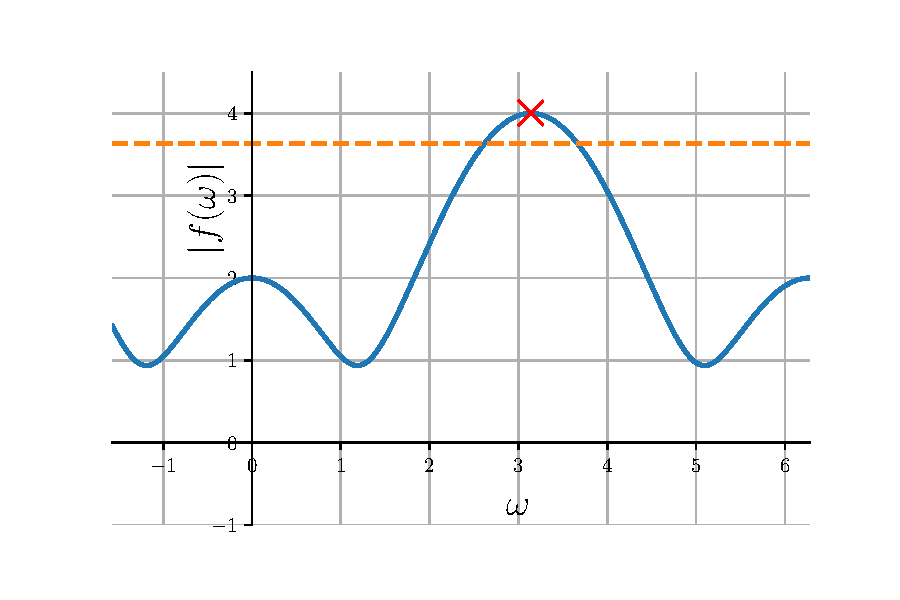
\includegraphics[scale=0.5]{images/graph_bound_gen_func/graph_n5.pdf}}\only<2>{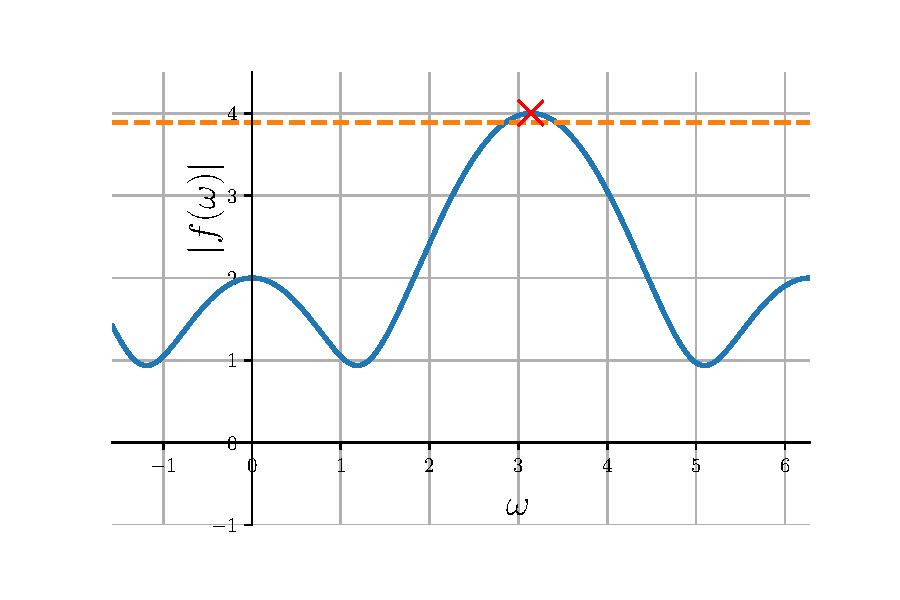
\includegraphics[scale=0.5]{images/graph_bound_gen_func/graph_n10.pdf}}\only<3>{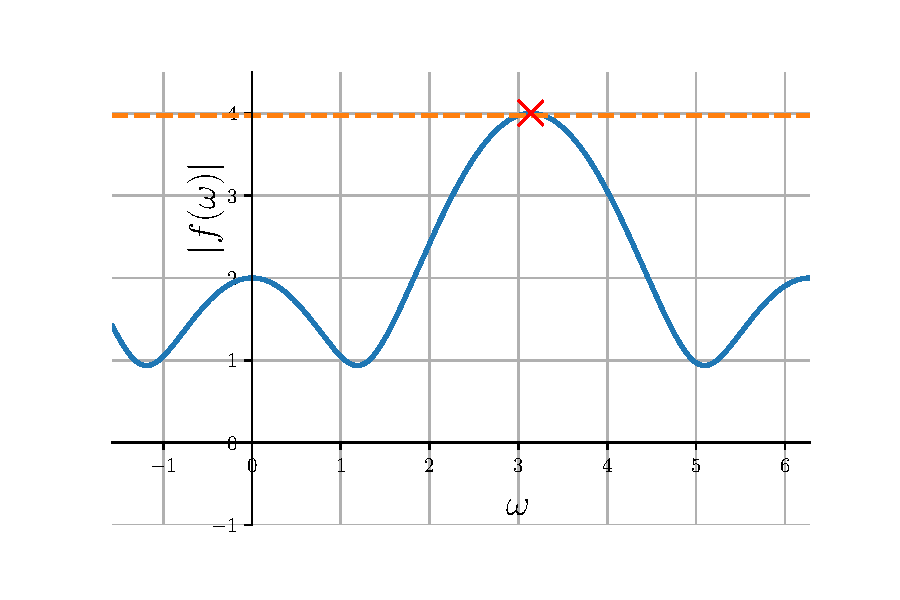
\includegraphics[scale=0.5]{images/graph_bound_gen_func/graph_n20.pdf}}
  \end{minipage}

  \def\point{10}
  \begin{tikzpicture}[overlay]
    \draw (9,3) node {{\color{darkblue}{$|f(\omega)|$}}};
    \visible<1>{  \draw (9.5,4.10) node {{\color{OrangePSL}{$\sigma_1(\Tmat) \approx 3.62$}}};}
    \visible<2>{  \draw (9.5,4.23) node {{\color{OrangePSL}{$\sigma_1(\Tmat) \approx 3.88$}}};}
    \visible<3->{ \draw (9.5,4.30) node {{\color{OrangePSL}{$\sigma_1(\Tmat) \approx 3.96$}}};}
  \end{tikzpicture}


\end{frame}





%%%%%%%%%%%%%%%%%%%%%%%%%%%%%%%%%%%%%%%%%%%%%%%%%%%%%%%%%%%%%%%%%%%%%%%%%%%%%%%
\begin{frame}{Equivalent Reasoning for Block Toeplitz Matrices}
%%%%%%%%%%%%%%%%%%%%%%%%%%%%%%%%%%%%%%%%%%%%%%%%%%%%%%%%%%%%%%%%%%%%%%%%%%%%%%%


  Let $g: [0, 2\pi] \rightarrow \Cbb^{m \times m}$ be a matrix-valued function and the inverse Fourier Transform of the sequence $\{ \Bsf_h \}_{\{-n+1, \dots, n-1\}}$:
  \begin{minipage}{\textwidth}
    \centering
    \begin{minipage}{0.45\textwidth}
      \begin{equation}
	  \Bmat = \scalebox{0.8}{
	  \begin{tikzpicture}[
	    baseline,
	    every left delimiter/.style={xshift=+0.78em},
	    every right delimiter/.style={xshift=-0.4em},
	    mymat/.style={
	      matrix of math nodes,
	      ampersand replacement=\&,
	      left delimiter=(,
	      right delimiter=),
	      nodes={
		text depth=0.5ex,
		text height=2ex,
		text width=2em,
		align=center}
	    }
	    ]
	    \matrix[mymat] (mytoeplitz) {
	       \Bsf_0  \& \Bsf_1 \& \cdots \& \Bsf_{n-1} \\
	       \Bsf_{-1} \& \color{black!30}{\Bsf_0} \& \color{black!30}{\ddots} \& \color{black!30}{\vdots} \\
	       \vdots  \& \color{black!30}{\ddots}  \& \color{black!30}{\Bsf_0}    \& \color{black!30}{\Bsf_1} \\
	       \Bsf_{-n+1} \& \color{black!30}{\cdots}  \& \color{black!30}{\Bsf_{-1}} \& \color{black!30}{\Bsf_0} \\
	    };
	  \end{tikzpicture}}
	  \phantom{ = \Amat}
      \end{equation}
    \end{minipage}
    \begin{minipage}{0.45\textwidth}
      \begin{equation}
	g(\omega) = \sum_{h = -n+1}^{n-1} \Bsf_h e^{\ci h \omega} 
      \end{equation}
    \end{minipage}
  \end{minipage}

  \begin{theorem}[{\color{SkyBlue}{\cite{gutierrez2012block}}}\xspace]
    Let $\Bmat$ a block Toeplitz matrix and $g$ the inverse Fourier transform of its associated sequence, then:
    \begin{equation}
      \sigma_1 \left( \Bmat \right) \leq \sup_{\omega \in [0, 2\pi]} \sigma_1 \left( g\left( \omega \right) \right)
    \end{equation}
  \end{theorem}

\end{frame}







%%%%%%%%%%%%%%%%%%%%%%%%%%%%%%%%%%%%%%%%%%%%%%%%%%%%%%%%%%%%%%%%%%%%%%%%%%%%%%%
\begin{frame}{Extension to Doubly-Block Toeplitz Matrices}
%%%%%%%%%%%%%%%%%%%%%%%%%%%%%%%%%%%%%%%%%%%%%%%%%%%%%%%%%%%%%%%%%%%%%%%%%%%%%%%

  \begin{minipage}{\textwidth}
    \centering
    We extend the reasoning to doubly-block Toeplitz matrices with \\ \orangebold{2d trigonometric polynomials}.
  \end{minipage}

  \vspace{0.3cm}
  \begin{itemize}
    \item[$\bullet$] <2-> The first dimension generates the block Toeplitz structure
    \item[$\bullet$] <3-> The second dimension generates the Toeplitz structure of each block
  \end{itemize}

  \vspace{0.5cm}
  \begin{overlayarea}{\textwidth}{2.8cm}
    \centering
    \only<2>{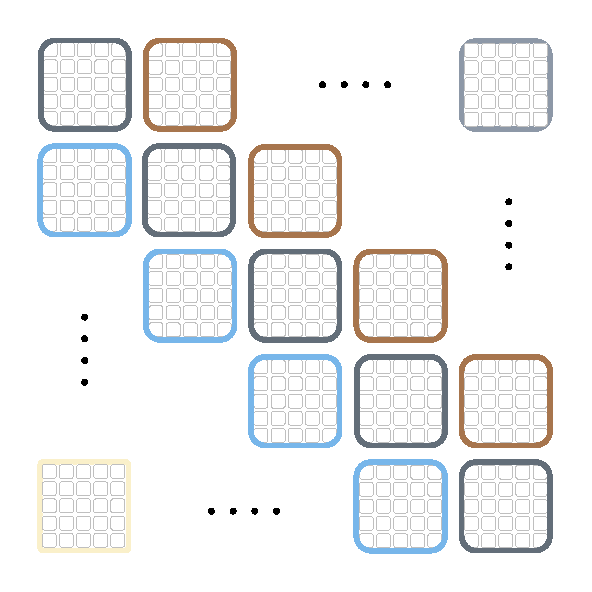
\includegraphics[scale=0.25]{images/doubly_block_v2.pdf}}\only<3->{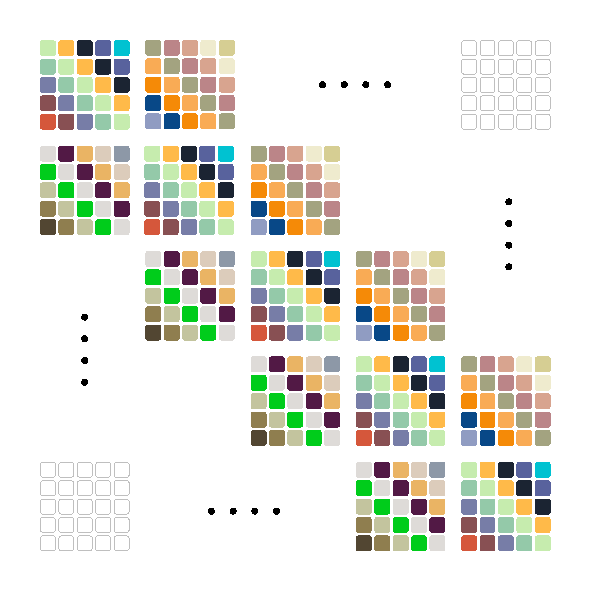
\includegraphics[scale=0.25]{images/doubly_block_v3.pdf}}
  \end{overlayarea}

\end{frame}




%%%%%%%%%%%%%%%%%%%%%%%%%%%%%%%%%%%%%%%%%%%%%%%%%%%%%%%%%%%%%%%%%%%%%%%%%%%%%%%
\begin{frame}{Bound on the Singular Values of Doubly-Block Toeplitz Matrices}
%%%%%%%%%%%%%%%%%%%%%%%%%%%%%%%%%%%%%%%%%%%%%%%%%%%%%%%%%%%%%%%%%%%%%%%%%%%%%%%

  In the same way as {\color{SkyBlue}{\cite{gray2006toeplitz}}}, we can bound the singular values of doubly-block Toeplitz matrices with their associated function.

  \visible<2->{
    \begin{theorem}[Bound on the singular values of a Doubly-Block Toeplitz]
      Let $\Dmat$ be a doubly-block Toeplitz matrix and $f$ its associated function, then:
      \vspace{-0.2cm}
      \begin{equation}
	\sigma_1 \left( \Dmat \right) \leq \sup_{\omega_1, \omega_2 \in [0, 2\pi]^2} |f(\omega_1,\omega_2)|
      \end{equation}
      \vspace{-0.2cm}
    \end{theorem}
  }

  \begin{itemize}
    \item[$\bullet$] <3-> Let $\phi$ be a convolution layer and $\Wmat$ the doubly-block Toeplitz equivalent to the convolution
    \item[$\bullet$] <4-> Let $f$ be the function associated with the matrix $\Wmat$
    \item[\orange{$\rightarrow$}] <5-> Then, we can upper bound the Lipschitz constant of the convolution:
      \begin{equation}
        \lip(\phi) \leq \sigma_1(\Wmat) \leq \sup_{\omega_1, \omega_2 \in [0, 2\pi]^2} |f(\omega_1,\omega_2)|
      \end{equation}
   \end{itemize}


\end{frame}


% %%%%%%%%%%%%%%%%%%%%%%%%%%%%%%%%%%%%%%%%%%%%%%%%%%%%%%%%%%%%%%%%%%%%%%%%%%%%%%%
% \begin{frame}{Convolution as Matrix-Multiplication}
% %%%%%%%%%%%%%%%%%%%%%%%%%%%%%%%%%%%%%%%%%%%%%%%%%%%%%%%%%%%%%%%%%%%%%%%%%%%%%%%
%   
%   % In practice, images has multiple \textbf{channels} (\eg RGB). We refer to the number of input channels $\cin$ and the number of output channels $\cout$.
%   In practice, images has multiple \textbf{channels}:
%   \vspace{-0.2cm}
%   \begin{itemize}
%     \item[$\bullet$] Input channels (\eg, RGB)
%     \item[$\bullet$] Output channels (number of convolution performed on the image)
%   \end{itemize}
%   \vspace{0.2cm}
%
%   \begin{minipage}{\textwidth}
%     \centering
%     \begin{minipage}{0.4\textwidth}
%       \centering
%       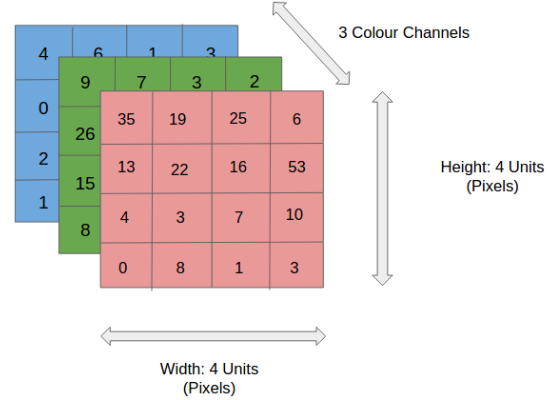
\includegraphics[scale=0.2]{images/image_rgb.png}
%     \end{minipage}
%     \begin{minipage}{0.4\textwidth}
%       \centering
%       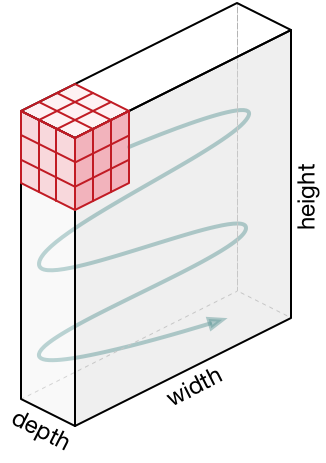
\includegraphics[scale=0.2]{images/conv_2d.png}
%     \end{minipage}
%   \end{minipage}
%
%   A multi-channel convolution is equivalent to a matrix-vector product where the matrix is a \textbf{block matrix} where each block is doubly-block Toeplitz matrix. 
%
% \end{frame}




%%%%%%%%%%%%%%%%%%%%%%%%%%%%%%%%%%%%%%%%%%%%%%%%%%%%%%%%%%%%%%%%%%%%%%%%%%%%%%%
\begin{frame}{Bound on the Singular Values of Convolution}
%%%%%%%%%%%%%%%%%%%%%%%%%%%%%%%%%%%%%%%%%%%%%%%%%%%%%%%%%%%%%%%%%%%%%%%%%%%%%%%
  

  \begin{minipage}{\textwidth}
    \centering
    \begin{minipage}{0.53\textwidth}
      In practice, images have multiple \textbf{channels}:
      {\small
      \begin{itemize}
	\item[$\bullet$] Input channels (\eg, RGB)
	\item[$\bullet$] Output channels (number of convolutions performed on the image)
      \end{itemize}
      }
    \end{minipage}
    \begin{minipage}{0.44\textwidth}
      \centering
      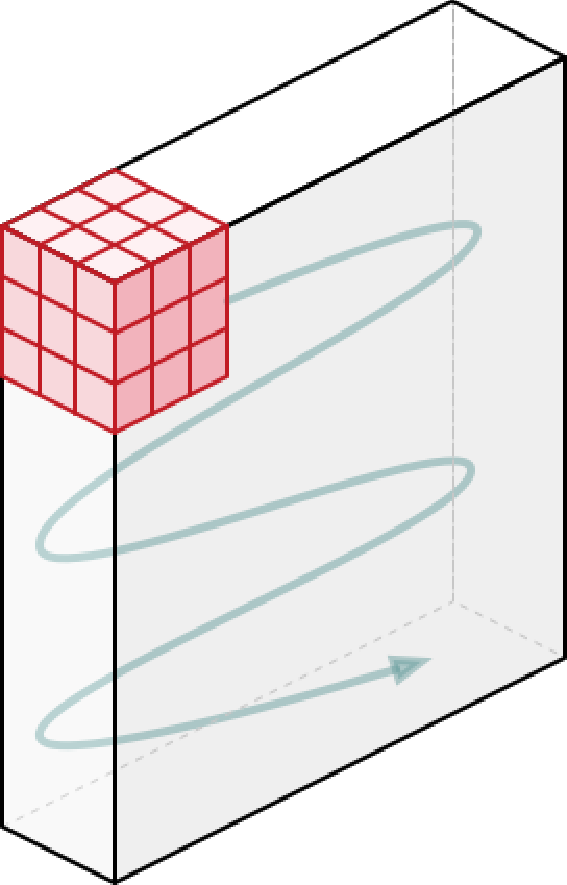
\includegraphics[scale=0.17]{images/conv_2d.pdf}
    \end{minipage}
  \end{minipage}


  \visible<2->{
    \begin{minipage}{\textwidth}
      \centering
      \begin{minipage}{0.49\textwidth}
	A multi-channel convolution is equivalent to a matrix-vector product where the matrix is a \textbf{block matrix} where each block is a doubly-block Toeplitz matrix. 
      \end{minipage}
      \begin{minipage}{0.49\textwidth}
	\centering
	\begin{equation}
	  \Mmat  = 
	    \scalebox{0.7}{
	    \begin{tikzpicture}[
	      baseline,
	      every left delimiter/.style={xshift=+0.78em},
	      every right delimiter/.style={xshift=-0.4em},
	      mymat/.style={
		matrix of math nodes,
		ampersand replacement=\&,
		left delimiter=(,
		right delimiter=),
		nodes={
		  text depth=0.5ex,
		  text height=2ex,
		  text width=3em,
		  align=center}
	      }
	      ]
	      \matrix[mymat] (matrix) {
		\Dmat_1\& \cdots \& \Dmat_{1,\cout} \\
		\vdots \& \& \vdots \\
		\Dmat_\cin \& \cdots \& \Dmat_{\cin,\cout} \\ 
	      };
	      \draw[decorate,decoration={mirror,raise=4pt},->] 
		($(matrix-1-3.north east)+(+0.4,0)$) -- node[above=4pt,sloped] 
		{Channels in}
		($(matrix-3-3.south east)+(+0.4,0)$);
	      \draw[decorate,decoration={mirror,raise=4pt},->] 
		($(matrix-1-1.north west)+(0,0.3)$) -- node[above=4pt,sloped] 
		{Channels out}
		($(matrix-1-3.north east)+(0,0.3)$);
	 \end{tikzpicture}}
	\end{equation}
       \end{minipage}
     \end{minipage}

    \begin{theorem}[Bound on the singular values of convolution]
      \begin{equation*}
	 \sigma_1(\Mmat) \leq \sqrt{ \sum_{i=1}^{\cout} \sup_{\omega_1, \omega_2 \in [0, 2\pi]^2} \sum_{j = 1}^{\cin} \left|f_{ij}(\omega_1, \omega_2) \right|^2 }  \triangleq \lipbound(\Mmat)
      \end{equation*}
    \end{theorem}
  }

\end{frame}






%%%%%%%%%%%%%%%%%%%%%%%%%%%%%%%%%%%%%%%%%%%%%%%%%%%%%%%%%%%%%%%%%%%%%%%%%%%%%%%
\begin{frame}{Tightness of LipBound}
%%%%%%%%%%%%%%%%%%%%%%%%%%%%%%%%%%%%%%%%%%%%%%%%%%%%%%%%%%%%%%%%%%%%%%%%%%%%%%%

  {\small
  \begin{itemize}
    \item[$\bullet$] The size of a matrix convolution is dependant on the size of the input
    \item[$\bullet$] When the size of the matrix increases, the associated function stays the same
  \end{itemize}
  }
  \vspace{-0.2cm}
  \begin{equation}
    \Gamma(n) = \lipbound(\Mmat(n)) - \sigma_1(\Mmat(n))
  \end{equation}
  \begin{minipage}{\textwidth}
    \centering
    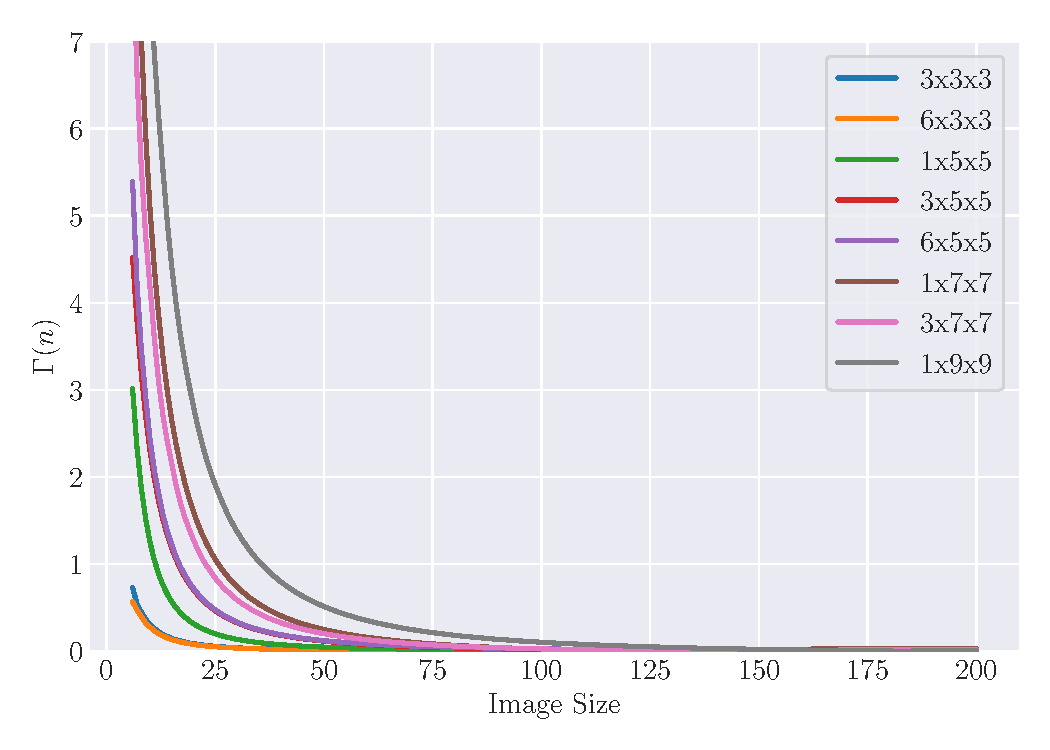
\includegraphics[scale=0.48]{images/convergence_bounds.pdf}
  \end{minipage}

\end{frame}


%%%%%%%%%%%%%%%%%%%%%%%%%%%%%%%%%%%%%%%%%%%%%%%%%%%%%%%%%%%%%%%%%%%%%%%%%%%%%%%
\begin{frame}{Computing LipBound}
%%%%%%%%%%%%%%%%%%%%%%%%%%%%%%%%%%%%%%%%%%%%%%%%%%%%%%%%%%%%%%%%%%%%%%%%%%%%%%%

  \begin{minipage}{\textwidth}
    \centering
    \begin{tabular}{cccc}
      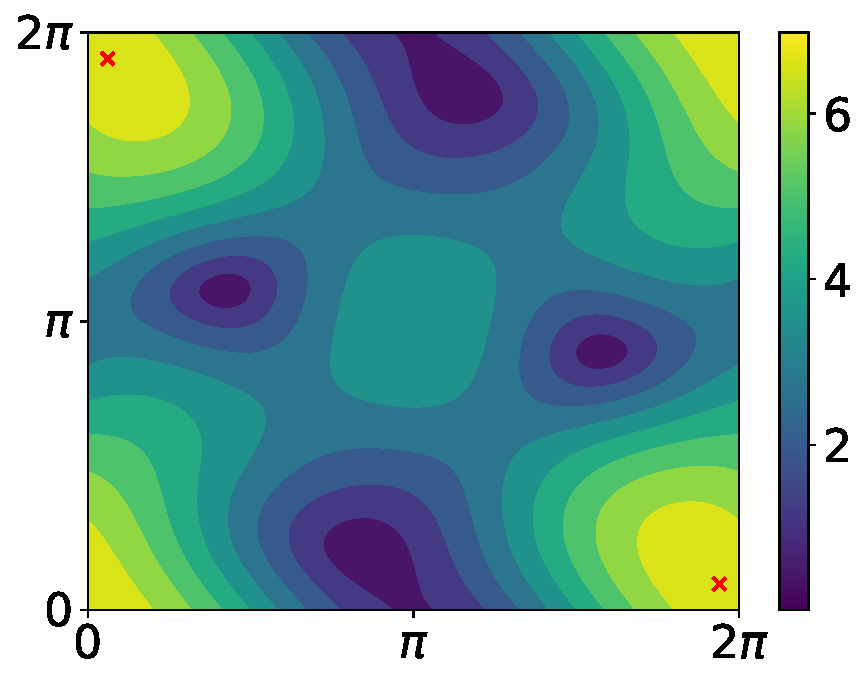
\includegraphics[scale=0.15]{images/contour_poly_200_1_1_3.pdf} &
      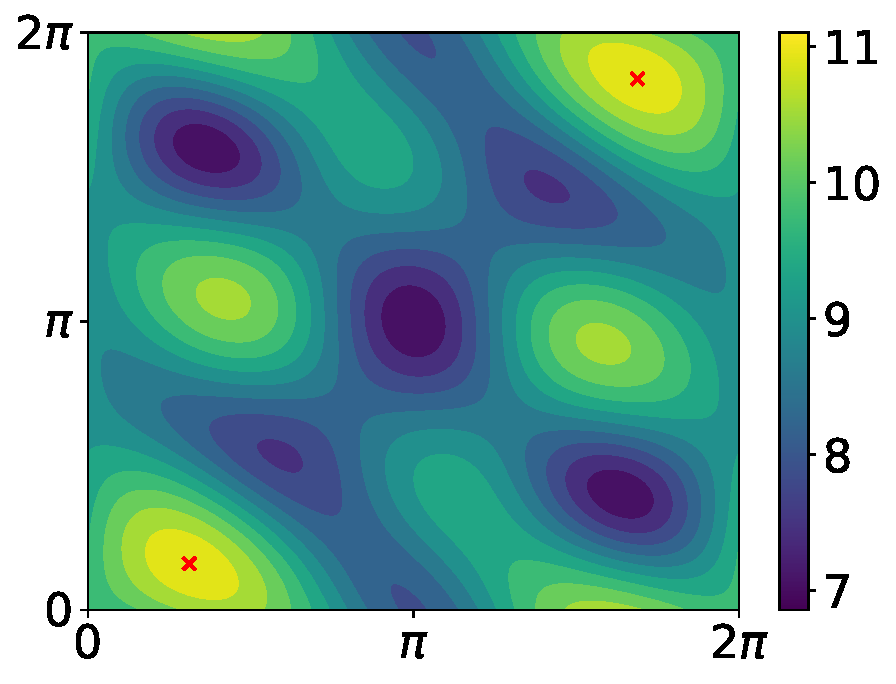
\includegraphics[scale=0.15]{images/contour_poly_200_1_9_3.pdf} & 
      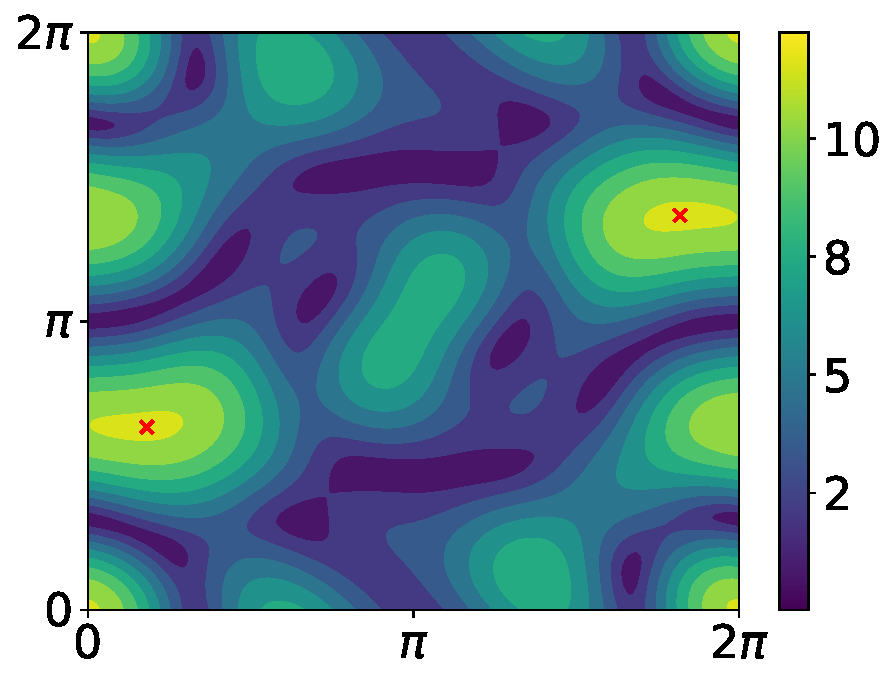
\includegraphics[scale=0.15]{images/contour_poly_200_1_1_5.pdf} & 
      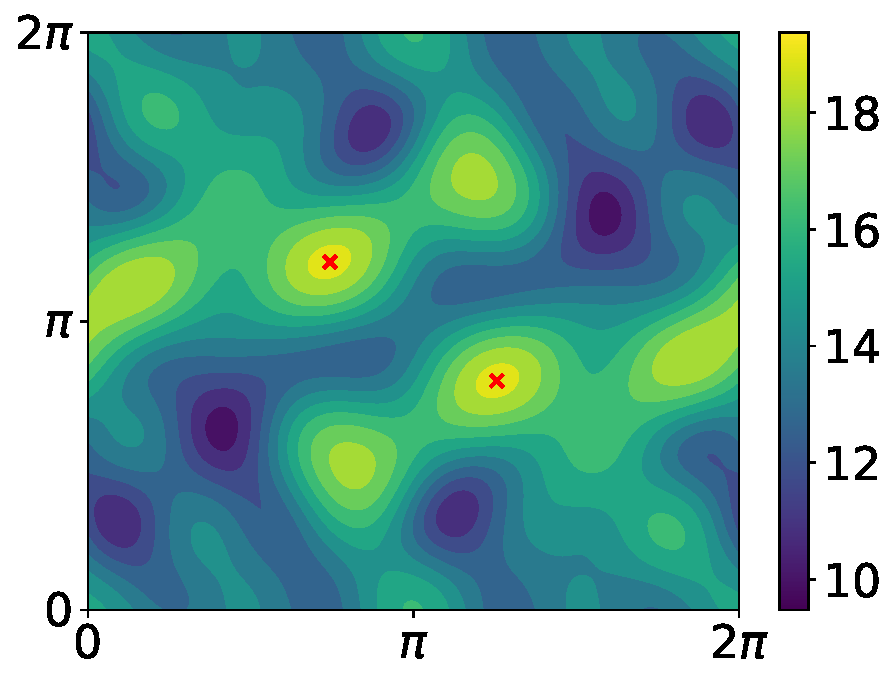
\includegraphics[scale=0.15]{images/contour_poly_200_1_9_5.pdf} \\
      \footnotesize{kernel $1\times3\times3$} &
      \footnotesize{kernel $9\times3\times3$} &
      \footnotesize{kernel $1\times5\times5$} &
      \footnotesize{kernel $9\times5\times5$}
    \end{tabular}

    \vspace{0.2cm}
    \footnotesize{Contour plot of multivariate trigonometric polynomials.}
  \end{minipage}

  \vspace{0.3cm}
  The computation of $\lipbound$ involves computing the maximum modulus of a 2-dimensional trigonometric polynomial on $[ 0, 2\pi]^2$.
  % Computing $\lipbound$ implies to compute the maximum modulus of a 2-dimensional trigonometric polynomial on 
  % $[ 0, 2\pi]^2$.

  \begin{itemize}
    \pause
  \item[$\bullet$] This problem has been known to be NP-hard ({\color{SkyBlue}{\cite{pfister2018bounding}}}).
    \pause
    \item[$\bullet$] However, trigonometric polynomials defined by usual convolutional kernels have a low degree (between 1 and 3)
    \pause
    \item[$\bullet$] A simple grid search algorithm is efficient and can be implemented on GPU
  \end{itemize}

\end{frame}


%%%%%%%%%%%%%%%%%%%%%%%%%%%%%%%%%%%%%%%%%%%%%%%%%%%%%%%%%%%%%%%%%%%%%%%%%%%%%%%
\begin{frame}{Precision of the Grid Search Algorithm}
%%%%%%%%%%%%%%%%%%%%%%%%%%%%%%%%%%%%%%%%%%%%%%%%%%%%%%%%%%%%%%%%%%%%%%%%%%%%%%%

  \begin{itemize}
    \item[$\bullet$] We can characterize the error of the grid search algorithm with respect to the number of samples $S$.
    \visible<2->{\item[$\bullet$] Let $f: [0, 2\pi]^2 \rightarrow \Cbb$ be a two dimensional trigonometric polynomial.}
  \end{itemize}

  \vspace{0.5cm}
  \begin{minipage}{\textwidth}
    \centering
    \begin{tabular}{ccc}
      \visible<2->{
      \begin{minipage}{0.2\textwidth}
	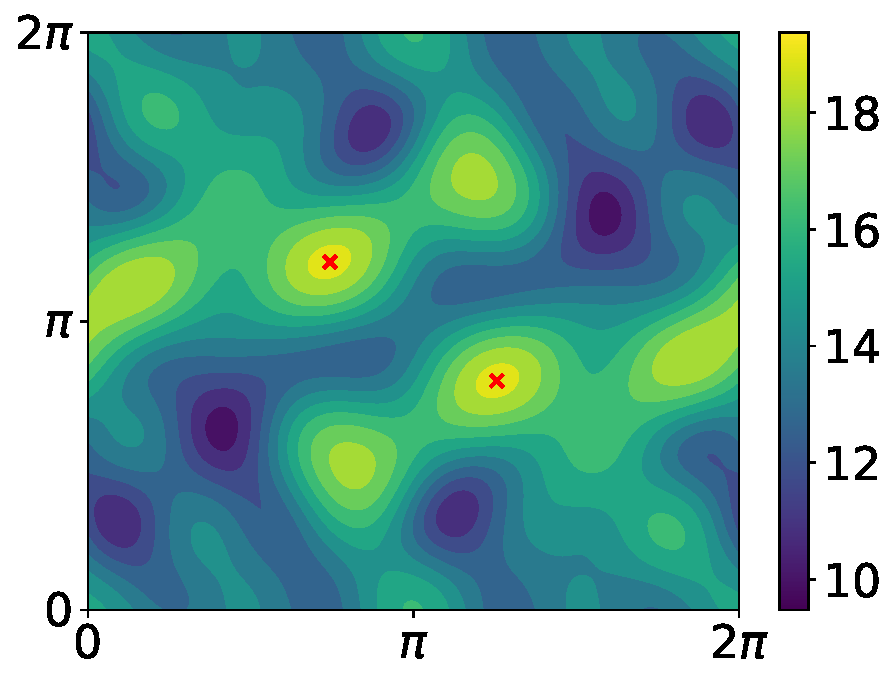
\includegraphics[scale=0.17]{images/contour_poly_200_1_9_5.pdf}
      \end{minipage}} & 
      \visible<3->{
      \begin{minipage}{0.2\textwidth}
	\centering
	$\underset{\text{discretization of}\atop\text{the search space}}{\Longrightarrow}$
      \end{minipage}} &
      \visible<3->{
      \begin{minipage}{0.2\textwidth}
	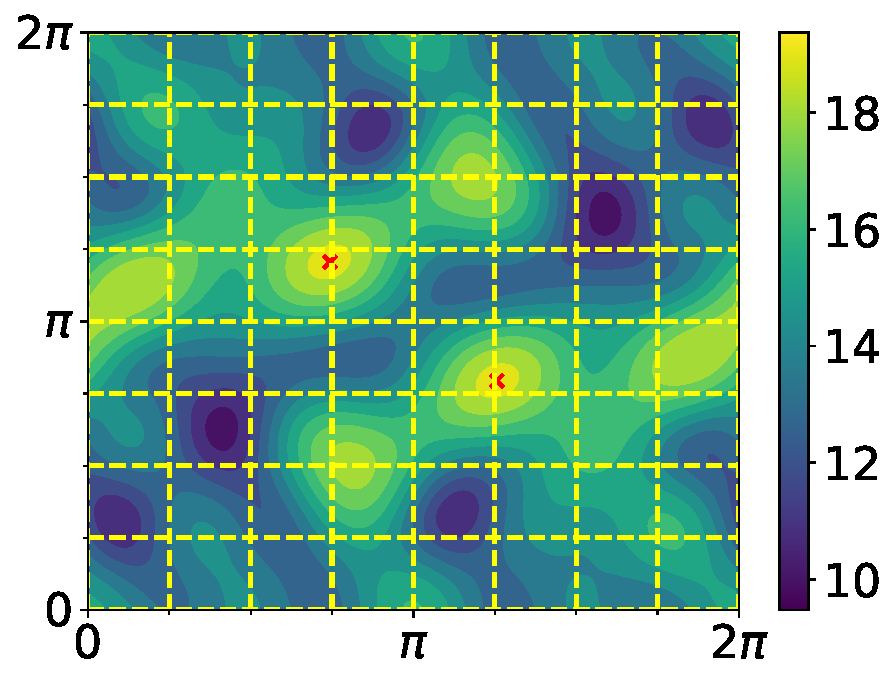
\includegraphics[scale=0.17]{images/contour_poly_200_1_9_5_grid.pdf}
      \end{minipage}} \\[1cm]
      \visible<2->{$\displaystyle \sup_{\omega_1, \omega_2 \in [0,2\pi]^2} \left| f(\omega_1, \omega_2) \right|$} & 
      \visible<4->{$\displaystyle \leq \frac{1}{(1 - \alpha)}$} &
      \visible<3->{$\displaystyle \max_{\omega_1', \omega_2' \in \Theta_S^2} \left| f(\omega_1', \omega_2') \right|$}
    \end{tabular}
  \end{minipage}

  \vspace{0.3cm}
  \visible<4->{
    \begin{itemize}
      \item where $\alpha = 2d/S$ is the degree of the polynomial \\
      \footnotesize{({\color{SkyBlue}{\cite{pfister2018bounding}}})}
    \end{itemize}
  }


\end{frame}



%%%%%%%%%%%%%%%%%%%%%%%%%%%%%%%%%%%%%%%%%%%%%%%%%%%%%%%%%%%%%%%%%%%%%%%%%%%%%%%
\subsection{Experiments}
%%%%%%%%%%%%%%%%%%%%%%%%%%%%%%%%%%%%%%%%%%%%%%%%%%%%%%%%%%%%%%%%%%%%%%%%%%%%%%%

% %%%%%%%%%%%%%%%%%%%%%%%%%%%%%%%%%%%%%%%%%%%%%%%%%%%%%%%%%%%%%%%%%%%%%%%%%%%%%%%
% \begin{frame}{Lipschitz Regularization of Convolutional Neural Networks}
% %%%%%%%%%%%%%%%%%%%%%%%%%%%%%%%%%%%%%%%%%%%%%%%%%%%%%%%%%%%%%%%%%%%%%%%%%%%%%%%
%  
%   We want to improve upon Adversarial Training:
%
%   \begin{equation}
%     \argmin_{h \in \Hcal} \ \frac{1}{m} \sum_{i = 1}^{m} \ell (h (\xvec_i + \tau^{\mathrm{adv}}(\xvec_i, y_i)), y_i) \color<1>{white}{ + \underbrace{{\color<3>{OrangePSL}{\lambda}} \sum_{j=1}^p \log(\lipbound(\Wmat^{(j)}))}_{\text{Our regularization}}}
%   \end{equation}
%
%   \visible<3->{
%     where {\color<3>{OrangePSL}{$\lambda$}} is user-defined parameter which controls the regularization.
%   }
%
%   \vspace{0.4cm}
%   \visible<4->{
%     $\Rightarrow$ Evaluation of the robustness with $l_2$ norm and several $\epsilon$
%   }
%
% \end{frame}


%%%%%%%%%%%%%%%%%%%%%%%%%%%%%%%%%%%%%%%%%%%%%%%%%%%%%%%%%%%%%%%%%%%%%%%%%%%%%%%
\begin{frame}{Lipschitz Regularization of Convolutional Neural Networks}
%%%%%%%%%%%%%%%%%%%%%%%%%%%%%%%%%%%%%%%%%%%%%%%%%%%%%%%%%%%%%%%%%%%%%%%%%%%%%%%
 
  We want to improve upon Adversarial Training:

  \begin{equation}
  \argmin_{h \in \Hcal} \ \frac{1}{m} \sum_{i = 1}^{m} \ell (h (\xvec_i + \tau^{\mathrm{adv}}(\xvec_i, y_i; h)), y_i)  + \underbrace{\lambda \sum_{j=1}^p \log(\lipbound(\Wmat^{(j)}))}_{\text{Our regularization}}
  \end{equation}
  where $\lambda$ is a user-defined parameter which controls the regularization.

  \vspace{0.4cm}
  $\Rightarrow$ Evaluation of the robustness with $l_2$ norm and several $\epsilon$

\end{frame}




% %%%%%%%%%%%%%%%%%%%%%%%%%%%%%%%%%%%%%%%%%%%%%%%%%%%%%%%%%%%%%%%%%%%%%%%%%%%%%%%
% \begin{frame}{Empirical Results}
% %%%%%%%%%%%%%%%%%%%%%%%%%%%%%%%%%%%%%%%%%%%%%%%%%%%%%%%%%%%%%%%%%%%%%%%%%%%%%%%
%
%   \begin{minipage}{\textwidth}
%     \centering
%     \small{
%     \begin{tabular}{lc}
%       \begin{tabular}{l}
% 	\orangebold{CIFAR10 Dataset $\quad$} \\
% 	50K images \\
% 	10 classes
%       \end{tabular}
%       &
%       \visible<2->{
%       \begin{tabular}{
% 	  M{l}{2-}
% 	  M{r}{2-}
% 	  M{r}{3-}
% 	  M{r}{4-}
% 	}
% 	\toprule
% 			   & \textbf{Accuracy}  & $\epsilon=0.6$ & $\epsilon = 0.8$ \\
% 	\midrule
%         \textbf{Baseline}  & \textbf{95}  & 0          & 0 \\
% 	\textbf{AT}        & 86           & 47          & 33 \\
% 	\textbf{AT+LipReg} & 80           & \textbf{54} & \textbf{43} \\
% 	\midrule
% 	  &  & +7 & +10 \\
% 	\bottomrule
%       \end{tabular}}
%      \end{tabular}
%      }
%   \end{minipage}
%
%
%
%   \vspace{0.8cm}
%   \visible<5->{
%   \begin{minipage}{\textwidth}
%     \centering
%     \small{
%      \begin{tabular}{lc}
% 	\begin{tabular}{l}
% 	  \orangebold{ImageNet Dataset $\quad$} \\
% 	  1.2M images \\
% 	  1000 classes
% 	\end{tabular}
%        &
%        \visible<6->{
%        \begin{tabular}{
% 	    M{l}{6-}
% 	    M{r}{6-}
% 	    M{r}{7-}
% 	    M{r}{8-}
%           }
% 	 \toprule
% 	   & \textbf{Accuracy} & $\epsilon=1$ & $\epsilon=2$ \\
% 	 \midrule
% 	 \textbf{Baseline}  & \textbf{78} & 0          & 0 \\
% 	 \textbf{AT}        & 50          & 30          & 16 \\
% 	 \textbf{AT+LipReg} & 51          & \textbf{33} & \textbf{20} \\
% 	 \midrule
% 	  & & +3 & +4 \\
% 	 \bottomrule
%        \end{tabular}}
%      \end{tabular}
%      }
%   \end{minipage}
%   }
%
% \end{frame}


%%%%%%%%%%%%%%%%%%%%%%%%%%%%%%%%%%%%%%%%%%%%%%%%%%%%%%%%%%%%%%%%%%%%%%%%%%%%%%%
\begin{frame}{Empirical Results}
%%%%%%%%%%%%%%%%%%%%%%%%%%%%%%%%%%%%%%%%%%%%%%%%%%%%%%%%%%%%%%%%%%%%%%%%%%%%%%%

  \begin{minipage}{\textwidth}
    \centering
    \small{
    \begin{tabular}{lc}
      \begin{tabular}{l}
	\orangebold{CIFAR10 Dataset $\quad$} \\
	50K images \\
	10 classes
      \end{tabular}
      &
      \begin{tabular}{lrrrr}
	\toprule
			   & \textbf{Accuracy}  & $\epsilon=0.6$ & $\epsilon = 0.8$ \\
	\midrule
        \textbf{Baseline}  & \textbf{95}  & 0          & 0 \\
	\textbf{AT}        & 86           & 47          & 33 \\
	\textbf{AT+LipReg} & 80           & \textbf{54} & \textbf{43} \\
	\midrule
	  &  & +7 & +10 \\
	\bottomrule
      \end{tabular}
     \end{tabular}
     }
  \end{minipage}



  \vspace{0.8cm}
  \visible<2->{
  \begin{minipage}{\textwidth}
    \centering
    \small{
     \begin{tabular}{lc}
	\begin{tabular}{l}
	  \orangebold{ImageNet Dataset $\quad$} \\
	  1.2M images \\
	  1000 classes
	\end{tabular}
       &
       \begin{tabular}{lrrr}
	 \toprule
	   & \textbf{Accuracy} & $\epsilon=1$ & $\epsilon=2$ \\
	 \midrule
	 \textbf{Baseline}  & \textbf{78} & 0          & 0 \\
	 \textbf{AT}        & 50          & 30          & 16 \\
	 \textbf{AT+LipReg} & 51          & \textbf{33} & \textbf{20} \\
	 \midrule
	  & & +3 & +4 \\
	 \bottomrule
       \end{tabular}
     \end{tabular}
     }
  \end{minipage}
  }

\end{frame}









